\documentclass{report}

\usepackage[margin=1in]{geometry}
\usepackage{amsmath,amsthm,amssymb}
\usepackage{enumitem}
\usepackage{graphicx}
\usepackage{caption}
\usepackage{mathtools}
\usepackage[obeyspaces,spaces]{url}
\usepackage{listings}
\usepackage{color}

\definecolor{dkgreen}{rgb}{0,0.6,0}
\definecolor{gray}{rgb}{0.5,0.5,0.5}
\definecolor{mauve}{rgb}{0.58,0,0.82}

\lstset{frame=tb,
  language=Java,
  aboveskip=3mm,
  belowskip=3mm,
  showstringspaces=false,
  columns=flexible,
  basicstyle={\small\ttfamily},
  numbers=none,
  numberstyle=\tiny\color{gray},
  keywordstyle=\color{blue},
  commentstyle=\color{dkgreen},
  stringstyle=\color{mauve},
  breaklines=true,
  breakatwhitespace=true,
  tabsize=3
}

\renewcommand{\familydefault}{\sfdefault}
\begin{document}
% ------------------------------------------ %
%                 START HERE                 %
% ------------------------------------------ %
\title{CS5785 Homework 2\\
\large{
    Applied Machine Learning
}
}


\author{
	Vijay Pillai\\
	Zachary Pardey}
\maketitle
\section*{Programming Exercises}

\begin{enumerate}
	\item Eigenface Method
	\begin{enumerate}[label=(\alph*)]
		\item See \path{./Faces/HW2_Q1_Faces.ipynb} for solution code.
		\item Pick a face image from X and display that image in grayscale. Do the same thing for the test set. \\
		The size of $X_{train}$ should be 540 × 2500.
		The size of matrix $X_{test}$ should be 100 × 2500.
		\begin{center}
		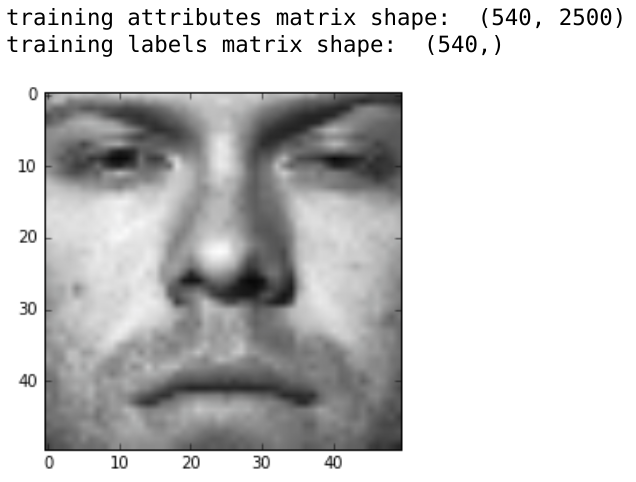
\includegraphics[width=6.75cm]{images/train_face.png}
		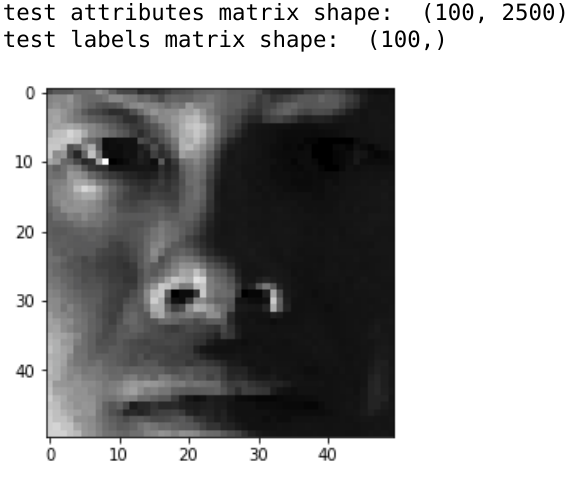
\includegraphics[width=6.1cm]{images/test_face.png}
		\end{center}
		\item Compute the average face μ from the whole training set by summing up every
column in X then dividing by the number of faces. Display the average face as a grayscale
image.
		\begin{center}
		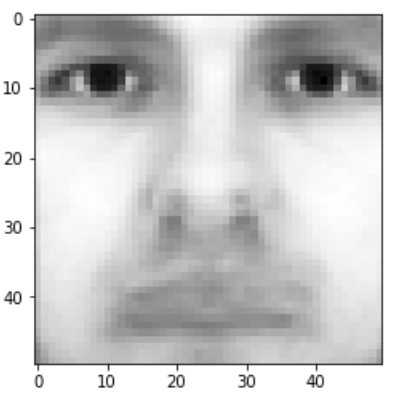
\includegraphics[width=7cm]{images/average_face.png}
		\end{center}
		\newpage
		\item Subtract average face $\mu$ from every column in $X$. Pick a face image after mean subtraction from the new $X$ and display that image in grayscale. Do the same thing for the test set $X_{test}$ using the pre-computed average face $\mu$ in (c).
		\begin{center}
		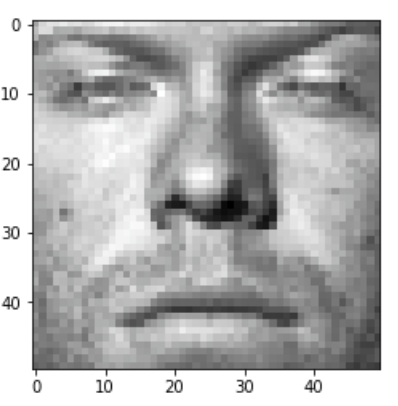
\includegraphics[width=6.5cm]{images/train_minus.png}
		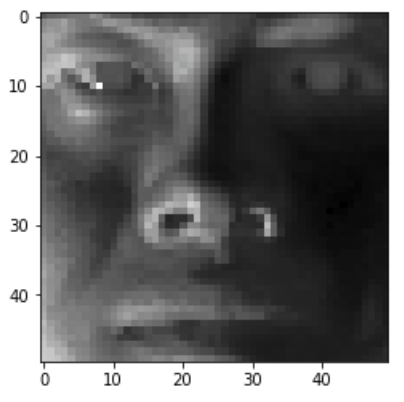
\includegraphics[width=6.5cm]{images/test_minus.png}
		\end{center}
		\item Perform Singular Value Decomposition (SVD) on the training set $X$ ($X = UΣV^{T} $) to get matrix $V^T$, where each row of $V^T$ has the same dimension as the face image... Display the first 10 eigenfaces as 10 images in grayscale. 
		\begin{center}
		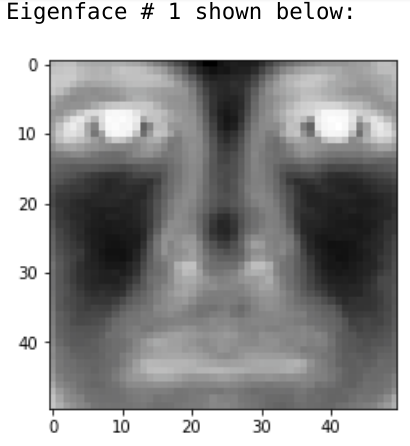
\includegraphics[width=4cm]{images/eface1.png}
		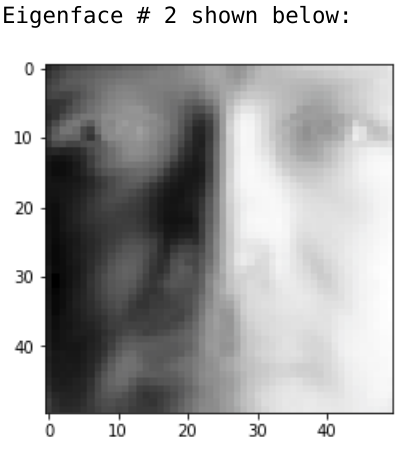
\includegraphics[width=4cm]{images/eface2.png}
		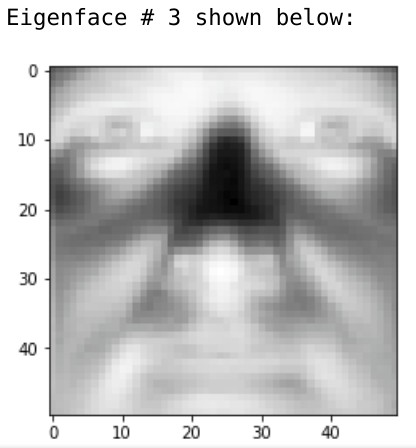
\includegraphics[width=4cm]{images/eface3.png}
		\end{center}
		See \path{./Faces/HW2_Q1_Faces.ipynb} for the remaining 10 faces.
		\newpage
		\item Plot the rank-r approximation error $||X - X̂_r||_F$ as a function of $r$ when $r = 1, 2, . . . , 200$. \\ 
		See file: \path{./Faces/HW2_Q1_Faces.ipynb} for source.\\
		\textit{x-axis: rank, y-axis: approximation error} 
		\begin{center}
		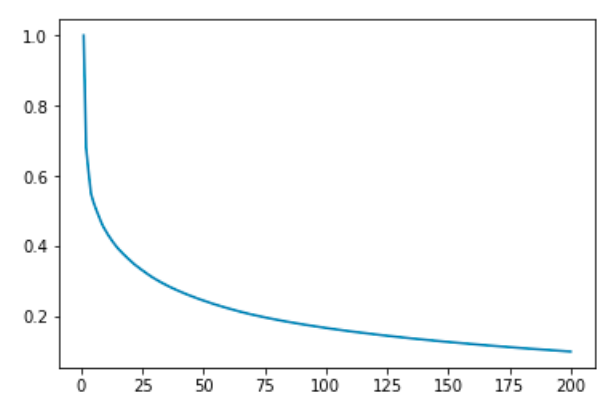
\includegraphics[width=10cm]{images/rank_error.png}
		\end{center}
		\item Write a function to generate r-dimensional feature
matrix $F$ and $F_{test}$ for training images $X$ and test images $X_{test}$, respectively. \\ \\
		See \path{./Faces/HW2_Q1_Faces.ipynb} for full context.
		\begin{lstlisting}
		def convert_dataset(data, r, V_tr):
    		lower_data = np.dot(data, np.transpose(V_tr[:r,:]))
    		return lower_data
		\end{lstlisting}
		\item Extract training and test features for $r = 10$. Train a Logistic Regression model using $F$ and test on $F_{test}$. Report the classification accuracy on the test set. Plot the classification accuracy on the test set as a function of $r$ when $r = 1, 2, . . . , 200$. Use “one-vs-rest” logistic regression, where a classifier is trained for each possible output label. \\ \\
		See file: \path{./Faces/HW2_Q1_Faces.ipynb} for source.\\
		\textit{Accuracy when $r=10$ is $0.84$.}
		\begin{center}
		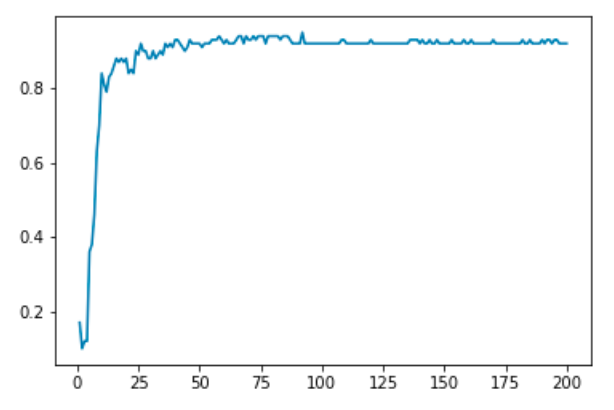
\includegraphics[width = 10cm]{images/accuracy.png}
		\end{center}
	\end{enumerate}
	
	\newpage
	
	\item Cooking
	\begin{enumerate}[label=(\alph*)]
		\item See \path{./Cooking/HW2_Q2_Cooking.ipynb} for solution code.
		\item Tell us about the data. How many samples (dishes) are there in the training set? How many categories (types of cuisine)? Use a list to keep all the unique ingredients appearing in the training set. How many unique ingredients are there? \\ \\
There are 39774 dishes in the dataset. \\
There are 6714 unique types of ingredients in the dataset. \\
There are 20 types of cuisine in the dataset.
		\item Represent each dish by a binary ingredient feature vector. Use $n*d$ feature matrix to represent all the dishes in training set and test set, where $n$ is the number of dishes.
		\\ \\
		Generated training feature matrix of shape: (39774, 6714). \\
		Generated test feature matrix of shape: (9944, 6714).
		\item Using Naïve Bayes Classifier to perform 3 fold cross-validation on the training set and report your average classification accuracy. Try both Gaussian distribution prior assumption and Bernoulli distribution prior assumption. \\ \\
		Naïve Bayes with Gaussian prior average classification accuracy: $0.379493793821$ \\
		Naïve Bayes with Bernoulli prior average classification accuracy: $0.683587657646$\\
		\item For Gaussian prior and Bernoulli prior, which performs better in terms of cross-validation accuracy? Why? Please give specific arguments. \\ \\
		The Bernoulli prior performs better in terms of cross-validation accuracy. This is because the Bernoulli is a discrete (binomial) distribution, while the Gaussian is a continuous distribution.  
Our feature matrix is modeled to better suit a discrete distribution, for each ingredient is modeled as a member of a discrete set, rather than a quantitative or continuous measure. Furthermore, food is discrete. An ingredient is not 90\% bananna, but either a bananna or not a bananna.  
Determining what kind of cuisine a food originated from based on the ingredients is thus based entirely on discrete probability.
		\item Using the Logistic Regression Model, perform 3 fold cross-validation on the training set and report your average classification accuracy. \\ \\
		Logistic Regression average accuracy: 0.7756
		\item Train your best-performed classifier with all of the training data, and generate test labels on test set. Submit your results to Kaggle and report the accuracy.
		\begin{center}
			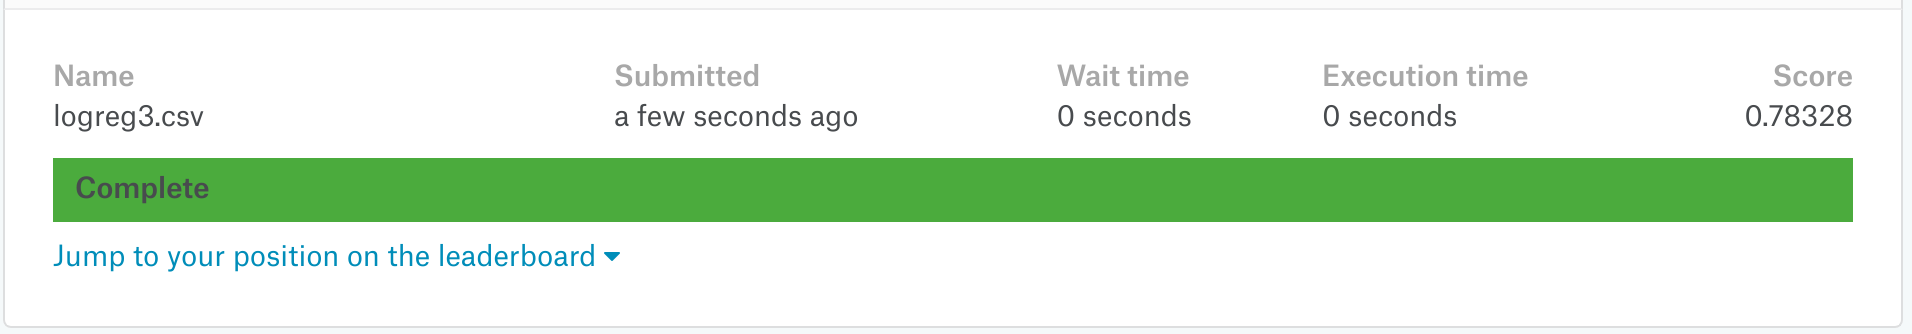
\includegraphics[width=15cm]{images/kaggle_score.png}
		\end{center}
		Note: the submission file was renamed to \path{./Cooking/submission.csv}
	\end{enumerate}
\end{enumerate}

\newpage

\section*{Written Exercises}	
\begin{enumerate}
\item HTF Exercise 4.1 \\
Show how to solve the generalized eigenvalue problem $max \ a^T \bold{B}a$
subject to $a^T\bold{W}a = 1$ by transforming to a standard eigenvalue problem. \\ \\
From HTF p.116:\\
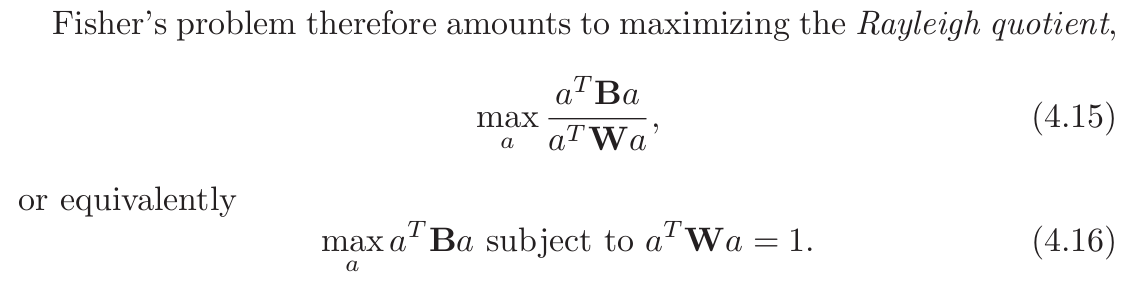
\includegraphics[width=10cm]{images/hint.png} \\
Therefore, use Lagrangian Optimization.
$L(a, \lambda)= (a^TBa)-\lambda(aWa-1)$ \\
\begin{align*}
\frac{\delta L}{\delta a} (a^TBa)-\lambda(aWa-1) &= 0 \\
2Ba+\lambda(2Wa) &= 0 \\
Ba + \lambda W a &= 0\\
W^{-1}(Ba+\lambda W a) &= 0\\
W^{-1}Ba &= \lambda a => Av = \lambda v\\
\end{align*}
This is the generalized eigenvalue problem. To solve the generalized eigenvalue problem, solve the characteristic polynomial for $\lambda$. \\
\begin{center}
$p(\lambda) = det(A-\lambda I)=0$ \\
\end{center}
\item HTF Exercise 4.2
	\begin{enumerate}
		\item 
		$
		\delta_2(x)>\delta_1(x) \\ 
		x^T \Sigma^{-1} \mu_2-\frac{1}{2} \mu_2^T \Sigma^{-1} \mu_2 + log(\frac{N_2}{N_{tot}}) > x^T \Sigma^{-1} \mu_1-\frac{1}{2} \mu_1^T + log(\frac{N_1}{N_{tot}})\\
		x^T \Sigma^{-1} \mu_2-X^T\Sigma^{-1} \mu_1 > \frac{1}{2} \mu_2^T \Sigma^{-1} \mu_2-\frac{1}{2} \mu_1^T \Sigma^{-1} \mu_1 + log(\frac{N_2}{N_{tot}})\\
		x^T \Sigma^{-1} \mu_2-X^T\Sigma^{-1} \mu_1 > \frac{1}{2} (\mu_2^T \Sigma^{-1} \mu_2-\frac{1}{2} \mu_1^T \Sigma^{-1} \mu_1) + log(\frac{N_1}{N_{tot}}-\frac{N_2}{N_{tot}})\\
		...\\
		\frac{1}{2} (\mu_2^T \Sigma^{-1} \mu_2-\frac{1}{2} \mu_1^T \Sigma^{-1} \mu_1) = (\mu_2+\mu_1)^T \Sigma^{-1}(\mu_2-\mu_1) \\
		...\\
		x^T \Sigma^{-1} (\mu_2 - \mu_1) > (\mu_2+\mu_1)^T \Sigma^{-1}(\mu_2-\mu_1) - log(\frac{N_2}{N_{1}})\\
		$
		\item no answer
		\item Show that $\Sigma_B \beta$ is in the direction $(\mu_2 - \mu_1)$ \\
		$\Sigma_B = \frac{N_1N_2}{N_2}(\mu_2-\mu_1)(\mu_2-\mu_1)^T$ \\
		$\Sigma_B \beta = \frac{N_1N_2}{N_2}(\mu_2-\mu_1)(\mu_2-\mu_1)^T \beta$\\
		$(\frac{N_1N_2}{N_2})(\mu_2-\mu_1)(\mu_2-\mu_1)^T \beta$\\
		...\\
		$(\frac{N_1N_2}{N_2})$ is scalar and $(\mu_2-\mu_1)^T \beta$ is scalar\\
		...\\
		$(\frac{N_1N_2}{N_2})(\mu_2-\mu_1)(\mu_2-\mu_1)^T \beta = (\mu_2-\mu_1) * scalar$ \\
		Thus, $\Sigma_B \beta$ is parallel to $(\mu_2 - \mu_1)$
		\item no answer
		\item no answer
	\end{enumerate}
\item SVD of Rank Deficient Matrix. Consider matrix $M$ . It has rank 2, as you can see by observing that there times the first column minus the other two columns is 0. \\
\begin{center}
$
M =
\begin{bmatrix}
    1&0&3 \\
    3&7&2 \\
    2&-2&8 \\
    0&-1&1 \\
    5&8&7 \\
\end{bmatrix}
$
\end{center}
	\begin{enumerate}
		\item Compute the matrices $M^TM$ and $MM^T$.\\ \\
		$
		M^T = 
		\begin{bmatrix}
    	1&3&2&0&5 \\
		0&7&-2&-1&8 \\
		3&2&8&1&7 \\
		\end{bmatrix}\\
		MM^T = 
		\begin{bmatrix}
		1&0&3 \\
		3&7&2 \\
		2&-2&8 \\
		0&-1&1 \\
		5&8&7 \\
		\end{bmatrix}
		\begin{bmatrix}
    	1&3&2&0&5 \\
		0&7&-2&-1&8 \\
		3&2&8&1&7 \\
		\end{bmatrix} = 
		\begin{bmatrix}
		10&9&26&3&26\\
		9&62&8&-5&85\\
		26&8&72&10&50\\
		3&-5&10&2&-1\\
		26&85&50&-1&138\\
  		\end{bmatrix}
		\\
		M^TM = 
		\begin{bmatrix}
    	1&3&2&0&5 \\
		0&7&-2&-1&8 \\
		3&2&8&1&7 \\
		\end{bmatrix}
		\begin{bmatrix}
		1&0&3 \\
		3&7&2 \\
		2&-2&8 \\
		0&-1&1 \\
		5&8&7 \\
		\end{bmatrix} = 
		\begin{bmatrix}
		39&57&60 \\
		57&118&53 \\
		60&53&127 \\
		\end{bmatrix}
		\\
		$
		\item Find the eigenvalues for your matrices of part (a). \\ \\
		$det(MM^T - \lambda I) = 0$ \\
		$\lambda_1 = 214.67$\\
		$\lambda_2 = 69.33$\\
		$\lambda_3 = 0$\\
		$\lambda_4 = 0$\\
		$\lambda_5 = 0$\\ \\
		$det(M^TM - \lambda I) = 0$\\
		$\lambda_1 = 214.67$\\
		$\lambda_2 = 69.33$\\
		$\lambda_3 = 0$\\
		\item Find the eigenvectors for the matrices of part (a). \\ \\
		For $\lambda_1 ... \lambda_5$: \\
		$MM^Tv = \lambda v$ \\
		$(MM^T - \lambda) v = 0$ \\
		$v_{1...5} = 
		\begin{bmatrix}
0.16492942 \\
0.47164732 \\
0.33647055 \\
0.00330585 \\
0.79820031 \\
		\end{bmatrix},
		\begin{bmatrix}
0.95539856 \\
0.03481209 \\
-0.27076072 \\
-0.04409532 \\
-0.10366268 \\
		\end{bmatrix},
		\begin{bmatrix}
-0.24497323 \\
0.45330644 \\
-0.82943965 \\
-0.16974659 \\
0.13310656 \\
		\end{bmatrix},
		\begin{bmatrix}
0.06456841 \\
-0.75012833 \\
-0.32834497 \\
-0.04619795 \\
0.56850131 \\
		\end{bmatrix},
		\begin{bmatrix}
-0.08432693 \\
0.16709883 \\
0.27420212 \\
-0.9233105 \\
-0.19307476 \\
		\end{bmatrix}
		$ \\ \\
		For $\lambda_1 ... \lambda_3$: \\
		$M^TMv = \lambda v$ \\
		$(M^TM - \lambda) v = 0$ \\
		$v_{1...3} = 
		\begin{bmatrix}
0.42615127 \\
0.61500884 \\
0.66344497 \\
		\end{bmatrix},
		\begin{bmatrix}
0.90453403 \\
-0.30151134 \\
-0.30151134 \\
		\end{bmatrix},
		\begin{bmatrix}
-0.01460404 \\
-0.72859799 \\
0.68478587 \\
		\end{bmatrix}
		$\\
		\item Find the SVD for the original matrix $M$ from parts (b) and (c). Note that there are only two nonzero eigenvalues, so your matrix $\Sigma$ should have only two singular values, while $U$ and $V$ have only two columns. \\ \\
		$X = UsV^T\\
		U = 
\begin{bmatrix}
0.16492942&-0.24497323&0.06456841\\
0.47164732&0.45330644&-0.75012833\\
0.33647055&-0.82943965&-0.32834497\\
0.00330585&-0.16974659&-0.04619795\\
0.79820031&0.13310656&0.56850131\\
\end{bmatrix}\\
s = 
\begin{bmatrix}
14.65163776&0&0\\
0&8.32643446&0\\
0&0&0\\
\end{bmatrix}\\
V^T = 
\begin{bmatrix}
0.42615127&0.61500884&0.66344497\\
-0.01460404&-0.72859799&0.68478587\\
0.90453403&-0.30151134&-0.30151134\\
\end{bmatrix}
$
		\item Set your smaller singular value to 0 and compute the one-dimensional approximation to the matrix $M$. \\ \\
		Rank 1 approximation: \\
$
X_1 = U_1 s_1 V^T_1 \\
X_1 = 
\begin{bmatrix}
0.16492942\\
0.47164732\\
0.33647055\\
0.00330585\\
0.79820031\\
\end{bmatrix}
\begin{bmatrix}
14.65163776\\
\end{bmatrix}
\begin{bmatrix}
0.42615127&0.61500884&0.66344497\\
\end{bmatrix}\\
X_1 = 
\begin{bmatrix}
1.02978864&1.48616035&1.60320558\\
2.94487812&4.24996055&4.58467382\\
2.10085952&3.031898&3.27068057\\
0.02064112&0.02978864&0.0321347\\
4.9838143&7.19249261&7.75895028\\
\end{bmatrix}
$
	\end{enumerate}
\end{enumerate}

\end{document}
 